\documentclass[a4paper]{jsarticle}
\setcounter{section}{2}
\setcounter{subsection}{0}
\usepackage{amsmath,amsfonts,amssymb,array,comment,mathtools,url,docmute}
\usepackage{longtable,booktabs,dcolumn,tabularx,mathtools,multirow,colortbl,xcolor}
\usepackage[dvipdfmx]{graphics}
\usepackage{bmpsize}
\usepackage{amsthm}
\usepackage{enumitem}
\setlistdepth{20}
\renewlist{itemize}{itemize}{20}
\setlist[itemize]{label=•}
\renewlist{enumerate}{enumerate}{20}
\setlist[enumerate]{label=\arabic*.}
\setcounter{MaxMatrixCols}{20}
\setcounter{tocdepth}{3}
\newcommand{\rotin}{\text{\rotatebox[origin=c]{90}{$\in $}}}
\newcommand{\amap}[6]{\text{\raisebox{-0.7cm}{\begin{tikzpicture} 
  \node (a) at (0, 1) {$\textstyle{#2}$};
  \node (b) at (#6, 1) {$\textstyle{#3}$};
  \node (c) at (0, 0) {$\textstyle{#4}$};
  \node (d) at (#6, 0) {$\textstyle{#5}$};
  \node (x) at (0, 0.5) {$\rotin $};
  \node (x) at (#6, 0.5) {$\rotin $};
  \draw[->] (a) to node[xshift=0pt, yshift=7pt] {$\textstyle{\scriptstyle{#1}}$} (b);
  \draw[|->] (c) to node[xshift=0pt, yshift=7pt] {$\textstyle{\scriptstyle{#1}}$} (d);
\end{tikzpicture}}}}
\newcommand{\twomaps}[9]{\text{\raisebox{-0.7cm}{\begin{tikzpicture} 
  \node (a) at (0, 1) {$\textstyle{#3}$};
  \node (b) at (#9, 1) {$\textstyle{#4}$};
  \node (c) at (#9+#9, 1) {$\textstyle{#5}$};
  \node (d) at (0, 0) {$\textstyle{#6}$};
  \node (e) at (#9, 0) {$\textstyle{#7}$};
  \node (f) at (#9+#9, 0) {$\textstyle{#8}$};
  \node (x) at (0, 0.5) {$\rotin $};
  \node (x) at (#9, 0.5) {$\rotin $};
  \node (x) at (#9+#9, 0.5) {$\rotin $};
  \draw[->] (a) to node[xshift=0pt, yshift=7pt] {$\textstyle{\scriptstyle{#1}}$} (b);
  \draw[|->] (d) to node[xshift=0pt, yshift=7pt] {$\textstyle{\scriptstyle{#2}}$} (e);
  \draw[->] (b) to node[xshift=0pt, yshift=7pt] {$\textstyle{\scriptstyle{#1}}$} (c);
  \draw[|->] (e) to node[xshift=0pt, yshift=7pt] {$\textstyle{\scriptstyle{#2}}$} (f);
\end{tikzpicture}}}}
\renewcommand{\thesection}{第\arabic{section}部}
\renewcommand{\thesubsection}{\arabic{section}.\arabic{subsection}}
\renewcommand{\thesubsubsection}{\arabic{section}.\arabic{subsection}.\arabic{subsubsection}}
\everymath{\displaystyle}
\allowdisplaybreaks[4]
\usepackage{vtable}
\theoremstyle{definition}
\newtheorem{thm}{定理}[subsection]
\newtheorem*{thm*}{定理}
\newtheorem{dfn}{定義}[subsection]
\newtheorem*{dfn*}{定義}
\newtheorem{axs}[dfn]{公理}
\newtheorem*{axs*}{公理}
\renewcommand{\headfont}{\bfseries}
\makeatletter
  \renewcommand{\section}{%
    \@startsection{section}{1}{\z@}%
    {\Cvs}{\Cvs}%
    {\normalfont\huge\headfont\raggedright}}
\makeatother
\makeatletter
  \renewcommand{\subsection}{%
    \@startsection{subsection}{2}{\z@}%
    {0.5\Cvs}{0.5\Cvs}%
    {\normalfont\LARGE\headfont\raggedright}}
\makeatother
\makeatletter
  \renewcommand{\subsubsection}{%
    \@startsection{subsubsection}{3}{\z@}%
    {0.4\Cvs}{0.4\Cvs}%
    {\normalfont\Large\headfont\raggedright}}
\makeatother
\makeatletter
\renewenvironment{proof}[1][\proofname]{\par
  \pushQED{\qed}%
  \normalfont \topsep6\p@\@plus6\p@\relax
  \trivlist
  \item\relax
  {
  #1\@addpunct{.}}\hspace\labelsep\ignorespaces
}{%
  \popQED\endtrivlist\@endpefalse
}
\makeatother
\renewcommand{\proofname}{\textbf{証明}}
\usepackage{tikz,graphics}
\usepackage[dvipdfmx]{hyperref}
\usepackage{pxjahyper}
\hypersetup{
 setpagesize=false,
 bookmarks=true,
 bookmarksdepth=tocdepth,
 bookmarksnumbered=true,
 colorlinks=false,
 pdftitle={},
 pdfsubject={},
 pdfauthor={},
 pdfkeywords={}}
\begin{document}
\subsection{集合}%\label{ux96c6ux5408}}
%\hypertarget{zfcux516cux7406ux7cfb}{%
\subsubsection{ZFC公理系}%\label{zfcux516cux7406ux7cfb}}
\begin{dfn}
集合論で扱われる以下に述べる公理たちを満たす対象のことを集合という\footnote{というか、この辺りではどっかの書籍を参考にしたというわけではなく、証明の行間も殆ど自分で埋めちゃったので、あんまりあてにしないほうがいいかもです…。}。
\end{dfn}
\begin{dfn}
集合論上の命題を作るために、新しい記号$\in$、$\ni$を導入しよう。命題$a \in A$を対象$a$は対象$A$の元である、対象$a$は対象$A$に属するという。命題$a \in A$を$A \ni a$とも書く。これの否定は$a \notin A$などと書かれる。
\end{dfn}
%\hypertarget{ux5916ux5ef6ux6027ux306eux516cux7406}{%
\subsubsection{外延性の公理}%\label{ux5916ux5ef6ux6027ux306eux516cux7406}}
\begin{axs}
次式で表される公理を外延性の公理などという。
\begin{align*}
\forall A,B\in \mathcal{F}\left[ A = B \Leftrightarrow \forall a \in A[a \in A \Leftrightarrow a \in B]\right]
\end{align*}
\end{axs}
これは集合$\mathcal{F}$に属する2つの集合たち$A$、$B$が式$A = B$を満たすならそのときに限り、その集合$A$の任意の元$a$がその集合$A$に属するならそのときに限り、その集合$B$にも属するという意味でありこれによってその式$A = B$を定めている。その式$A = B$をその集合$A$とその集合$B$は等しい、その集合$A$はその集合$B$に等しいという。簡単にいえば、$\forall a \in A$に対し、$a \in A$が成り立つならそのときに限り、$a \in B$が成り立つことを$A = B$が成り立つとしている。
\begin{dfn}
次式が成り立つとき、その集合$A$はその集合$B$に含まれる、その集合$B$はその集合$A$を含む、その集合$B$はその集合$A$を包む、その集合$B$はその集合$A$の部分集合であるといい、$A \subseteq B$、$B \supseteq A$などと書く。
\begin{align*}
\forall A,B\in \mathcal{F}\left[ A \subseteq B \Leftrightarrow \forall a \in A[a \in A \Rightarrow a \in B ]\right]
\end{align*}
\end{dfn}
簡単にいえば、$\forall a \in A$に対し、$a \in A$が成り立つなら、$a \in B$が成り立つことを$A \subseteq B$が成り立つとしている。
\begin{dfn}
次式が成り立つとき、その集合$B$はその集合$A$の真部分集合であるといい、$A \subset B$、$B \supset A$などと書く。
\begin{align*}
    \forall A,B\in \mathcal{F}[ A \subset B \Leftrightarrow A \subseteq B \land A \neq B]
\end{align*}
\end{dfn}
ただし、式々$A \subseteq B$、$A \subset B$をしばしば$A \subset B、A \subsetneq B$などと書く場合もあることに注意されたい。簡単にいえば、$A \subseteq B$が成り立つかつ、$A = B$が成り立たないことを$A \subset B$が成り立つとしている。
%\hypertarget{ux7a7aux96c6ux5408ux306eux516cux7406}{%
\subsubsection{空集合の公理}%\label{ux7a7aux96c6ux5408ux306eux516cux7406}}
\begin{axs}
次式で表される公理を空集合の公理、空集合の存在公理などという。
\begin{align*}
\exists A\in \mathcal{F}\forall B\in \mathcal{F} \forall a \in B[ a \notin A]
\end{align*}
\end{axs}
これは集合$\mathcal{F}$に属する集合$B$に属するどの集合$a$が属さないような集合$\mathcal{F}$に属する集合$A$が存在する、即ち、集合$\mathcal{F}$に属するどの集合$B$を選んでも、その集合$A$に属するような集合$B$の元$a$が存在できないようなその集合$\mathcal{F}$に属する集合$A$が存在することができるという意味であり、これによりその集合$A$を定めている。これを空集合といい、のちに述べるようにその存在は一意的なので、$\emptyset$と書く。
\begin{thm}
\label{1.2.1.1}
集合$A$が空集合であるならそのときに限り、その集合$A$がその集合$A$が属する集合$\mathcal{F}$のどの元$B$の部分集合である、即ち、次式が成り立つ。
\begin{align*}
\forall B\in \mathcal{F} \forall a \in B[ a \notin A] \Leftrightarrow \forall B\in \mathcal{F}[ A \subseteq B]
\end{align*}
\end{thm}
\begin{proof}
$\forall B\in \mathcal{F} \forall a \in B[ a \notin A]$より$a \in B \vee a \notin A$、即ち、$a \notin B \Rightarrow a \notin A$が成り立ち、対偶律により$A \subseteq B$が成り立つ。また、$\forall B\in \mathcal{F}[ A \subseteq B]$なる集合$A$を考えると、$A \subseteq B$が得られるが、対偶律より$a \notin B \Rightarrow a \notin A$が成り立ち$\forall B\in \mathcal{F} \forall a \in B[ a \notin A]$が得られる。
\end{proof}
\begin{thm}
\label{1.2.1.2}
空集合は一意的である。
\end{thm}
\begin{proof}
2つの異なる集合たち$B$、$C$がどちらも空集合であれば、定理\refeq{1.2.1.1}よりそれらの集合たち$B$、$C$がそれらの集合たち$B$、$C$が属する集合$\mathcal{F}$のどの元$A$の部分集合であることになり$\forall A\in \mathcal{F}[ B \subseteq A \land C \subseteq A]$が成り立ち、したがって、$B \subseteq C$かつ$C \subseteq B$が得られ$B = C$が得られるが、これは仮定に矛盾する。よって、空集合は一意的である。
\end{proof}
%\hypertarget{ux5bfeux306eux516cux7406}{%
\subsubsection{対の公理}%\label{ux5bfeux306eux516cux7406}}
\begin{axs} 
次式で表される公理を対の公理、非順序対の存在公理などという。
\begin{align*}
\forall A\in \mathcal{F} \forall a,b \in A\exists B\in \mathcal{F} \forall c \in B[ c \in B \Leftrightarrow c = a \vee c = b]
\end{align*}
\end{axs}
これは集合$\mathcal{F}$に属する任意の集合$A$に属する集合たち$a$、$b$を用いてその集合$\mathcal{F}$に属する集合$B$に属する集合$c$がそれらの集合たち$a$、$b$のいづれかになれるようなその集合$B$が存在できるという意味でありこの集合$B$をそれらの集合たち$a$、$b$の非順序対といい$\left\{ a,b \right\}$と書き、特に、集合$\left\{ a,a \right\}$を$\left\{ a \right\}$と書く。この公理によってその記法が定められ、その記法を外延的記法という。
\begin{thm}
\label{1.2.1.3}
次のことが成り立つ。
\begin{itemize}
\item
  $\forall A\in \mathcal{F} \forall a,b \in A$に対し、$\left\{ a,b \right\} = \left\{ b,a \right\}$が成り立つ。
\item
  $\forall A\in \mathcal{F} \forall a,b \in A$に対し、$a \in \left\{ b \right\}$が成り立つならそのときに限り、$a = b$が成り立つ。
\end{itemize}
\end{thm}
\begin{proof}
$\forall A\in \mathcal{F} \forall a,b \in A\forall c \in \left\{ a,b \right\}$に対し、次のようになる。
\begin{align*}
c \in \left\{ a,b \right\} &\Leftrightarrow c = a \vee c = b \\ 
&\Leftrightarrow c = b \vee c = a \\
&\Leftrightarrow c \in \left\{ b,a \right\}
\end{align*}
したがって、外延性の公理より次式が成り立つ。
\begin{align*}
\left\{ a,b \right\} = \left\{ b,a \right\}
\end{align*}
$\forall A\in \mathcal{F} \forall a,b \in A$に対し、$\left\{ b \right\} = \left\{ b,b \right\}$より次のようになる。
\begin{align*}
a \in \left\{ b \right\} = \left\{ b,b \right\} &\Leftrightarrow a = b \vee a = b \\ 
&\Leftrightarrow a = b
\end{align*}
\end{proof}
%\hypertarget{ux548cux96c6ux5408ux306eux516cux7406}{%
\subsubsection{和集合の公理}%\label{ux548cux96c6ux5408ux306eux516cux7406}}
\begin{axs}\label{和集合の公理}
次式で表される公理を和集合の公理、合併集合の存在公理などという。
\begin{align*}
\forall\mathcal{A}\in \mathcal{F\exists}A \in \mathcal{G\forall}a \in A\left[ a \in A \Leftrightarrow \exists B \in \mathcal{A}[ a \in B] \right]
\end{align*}
\end{axs}
これは、任意の集合$\mathcal{A}$に対し、集合$A$が存在して、任意の集合$a$に対し、その集合$a$がその集合$A$に属することとその集合$a$がその集合$\mathcal{A}$に属するある集合$B$に属することと同値であるという意味である。これにより、その集合$A$はその集合$\mathcal{A}$の元々の元々全体からなる集合となる。
\begin{thm}
\label{1.2.1.4}
その集合$A$は一意的である。
\end{thm}
\begin{proof}
このような異なる2つの集合たち$A$、$B$が与えられたとき、変数の現れに注意すれば、$\forall a \in A\left[ a \in A \Leftrightarrow \exists C \in \mathcal{A}[ a \in C] \Leftrightarrow a \in B \right]$が得られ外延性の公理より$A = B$が成り立つが、これは仮定に矛盾する。
\end{proof}
\begin{dfn}
この集合$A$をその集合$\mathcal{A}$に属する集合たち全体の和集合、合併、合併集合などといい、$\bigcup_{B \in \mathcal{A}} B$、$\bigcup_{} \mathcal{A}$、$\bigcup_{\mathcal{A}} $などと書く。特に、$\mathcal{A} =\left\{ A,B \right\}$が成り立つとき、和集合$\bigcup_{} \mathcal{A}$を$A \cup B$などと書く。
\end{dfn}
\begin{thm}
\label{1.2.1.5}
次のことが成り立つ。
\begin{itemize}
\item
  $\forall a \in \bigcup_{A \in \mathcal{A}} A$に対し、$a \in \bigcup_{A \in \mathcal{A}} A$が成り立つならそのときに限り、$\exists A \in \mathcal{A}$に対し、$a \in A$が成り立つ。
\item
  $\forall a \in A \cup B$に対し、$a \in A \cup B$が成り立つならそのときに限り、$a \in A$または$a \in B$が成り立つ。
\end{itemize}
\end{thm}
\begin{proof}
和集合の公理より明らかである。後半については次の通りである。
\begin{align*}
a \in A \cup B &\Leftrightarrow \exists C \in \left\{ A,B \right\}[ a \in C] \\
&\Leftrightarrow \left( A \in \left\{ A,B \right\} \land a \in A \right) \vee \left( B \in \left\{ A,B \right\} \land a \in B \right) \\
&\Leftrightarrow (\top \land a \in A) \vee (\top \land a \in B) \\
&\Leftrightarrow a \in A \vee a \in B
\end{align*}
\end{proof}
\begin{thm}
\label{1.2.1.6}
$\left\{ a,b \right\} = \left\{ a \right\} \cup \left\{ b \right\}$が成り立つ。
\end{thm}
\begin{proof}
$\forall c \in \left\{ a \right\} \cup \left\{ b \right\}$に対し、次のようになる。
\begin{align*}
c \in \left\{ a \right\} \cup \left\{ b \right\} \Leftrightarrow c \in \left\{ a \right\} \vee c \in \left\{ b \right\} \Leftrightarrow c = a \vee c = b \Leftrightarrow c \in \left\{ a,b \right\}
\end{align*}
\end{proof}
\begin{thm}
\label{1.2.1.7}
4つの集合たち$a_{1}$、$a_{2}$、$b_{1}$、$b_{2}$について次のことが成り立つ。
\begin{itemize}
\item
  $\left\{ a_{1},b_{1} \right\} = \left\{ a_{2},b_{2} \right\}$が成り立つならそのときに限り、$\left( a_{1} = a_{2} \land b_{1} = b_{2} \right) \vee \left( a_{1} = b_{2} \land b_{1} = a_{2} \right)$が成り立つ。
\item
  $\left\{ a \right\} = \left\{ b_{1},b_{2} \right\}$が成り立つならそのときに限り、$a = b_{1} = b_{2}$が成り立つ。
\end{itemize}
\end{thm}
\begin{proof}
4つの集合たち$a_{1}$、$a_{2}$、$b_{1}$、$b_{2}$について外延性の公理より次のようになる。
\begin{align*}
\left\{ a_{1},b_{1} \right\} = \left\{ a_{2},b_{2} \right\} \Leftrightarrow \forall a \in \left\{ a_{1},b_{1} \right\}\left[ a \in \left\{ a_{1},b_{1} \right\} \Leftrightarrow a \in \left\{ a_{2},b_{2} \right\} \right]
\end{align*}
ここで、次のようになるので、
\begin{align*}
\left( a \in \left\{ a_{1},b_{1} \right\} \Leftrightarrow a \in \left\{ a_{2},b_{2} \right\} \right) &\Leftrightarrow \left( a \in \left\{ a_{1},b_{1} \right\} \Leftrightarrow a \in \left\{ a_{2} \right\} \cup \left\{ b_{2} \right\} \right) \\
&\Leftrightarrow \left( a \in \left\{ a_{1},b_{1} \right\} \Leftrightarrow a \in \left\{ a_{2} \right\} \vee a \in \left\{ b_{2} \right\} \right) \\
&\Leftrightarrow \left( a \in \left\{ a_{1},b_{1} \right\} \Leftrightarrow a = a_{2} \vee a = b_{2} \right) \\
&\Leftrightarrow \neg\left( a \in \left\{ a_{1},b_{1} \right\} \vee \left( a = a_{2} \vee a = b_{2} \right) \right) \\
&\quad \vee \left( a \in \left\{ a_{1},b_{1} \right\} \land \left( a = a_{2} \vee a = b_{2} \right) \right) \\
&\Leftrightarrow \neg\left( \top \vee \left( a = a_{2} \vee a = b_{2} \right) \right) \\
&\quad \vee \left( \left( a = a_{2} \vee a = b_{2} \right) \land \top \right) \\
&\Leftrightarrow \bot \vee \left( a = a_{2} \vee a = b_{2} \right) \\
&\Leftrightarrow a = a_{2} \vee a = b_{2}
\end{align*}
次のようになる。
\begin{align*}
\left\{ a_{1},b_{1} \right\} = \left\{ a_{2},b_{2} \right\} &\Leftrightarrow \forall a \in \left\{ a_{1},b_{1} \right\}\left[ a = a_{2} \vee a = b_{2} \right] \\
&\Leftrightarrow \left( a_{1} = a_{2} \vee a_{1} = b_{2} \right) \land \left( b_{1} = a_{2} \vee b_{1} = b_{2} \right) \\
&\Leftrightarrow \left( a_{1} = a_{2} \land b_{1} = a_{2} \right) \vee \left( a_{1} = a_{2} \land b_{1} = b_{2} \right) \\ 
&\quad \vee \left( a_{1} = b_{2} \land b_{1} = a_{2} \right) \vee \left( a_{1} = b_{2} \land b_{1} = b_{2} \right) \\
&\Leftrightarrow \left( a_{1} = a_{2} = b_{1} \right) \vee \left( a_{1} = b_{1} = b_{2} \right) \\
&\quad \vee \left( a_{1} = b_{2} \land b_{1} = a_{2} \right) \vee \left( a_{1} = b_{2} \land b_{1} = b_{2} \right) \\
&\Leftrightarrow \left( a_{1} = a_{2} = b_{1} \land \left( b_{2} = a_{1} \vee b_{2} = b_{1} \right) \right) \\ 
&\quad \vee \left( a_{1} = b_{1} = b_{2} \land \left( a_{2} = a_{1} \vee a_{2} = b_{1} \right) \right) \\
&\quad \vee \left( a_{1} = b_{2} \land b_{1} = a_{2} \right) \vee \left( a_{1} = b_{2} \land b_{1} = b_{2} \right) \\
&\Leftrightarrow \left( a_{1} = a_{2} = b_{1} \land b_{2} = a_{1} \right) \vee \left( a_{1} = a_{2} = b_{1} \land b_{2} = b_{1} \right) \\
&\quad \vee \left( a_{1} = b_{1} = b_{2} \land a_{2} = a_{1} \right) \vee \left( a_{1} = b_{1} = b_{2} \land a_{2} = b_{1} \right) \\
&\quad \vee \left( a_{1} = b_{2} \land b_{1} = a_{2} \right) \vee \left( a_{1} = b_{2} \land b_{1} = b_{2} \right) \\
&\Leftrightarrow \left( a_{1} = a_{2} = b_{1} = b_{2} \right) \vee \left( a_{1} = b_{2} \land b_{1} = a_{2} \right) \\
&\quad \vee \left( a_{1} = b_{2} \land b_{1} = b_{2} \right) \\
&\Leftrightarrow \left( a_{1} = b_{2} \land b_{1} = a_{2} \land b_{1} = b_{2} \right) \vee \left( a_{1} = b_{2} \land b_{1} = a_{2} \right) \\
&\quad \vee \left( a_{1} = b_{2} \land b_{1} = b_{2} \land b_{1} = b_{2} \right) \vee \left( a_{1} = b_{2} \land b_{1} = b_{2} \right) \\
&\Leftrightarrow \left( a_{1} = b_{2} \land b_{1} = a_{2} \land \left( b_{1} = b_{2} \vee \top \right) \right) \\
&\quad \vee \left( a_{1} = b_{2} \land b_{1} = b_{2} \land \left( b_{1} = b_{2} \vee \top \right) \right) \\
&\Leftrightarrow \left( a_{1} = b_{2} \land b_{1} = a_{2} \land \top \right) \vee \left( a_{1} = b_{2} \land b_{1} = b_{2} \land \top \right) \\
&\Leftrightarrow \left( a_{1} = a_{2} \land b_{1} = b_{2} \right) \vee \left( a_{1} = b_{2} \land b_{1} = a_{2} \right)
\end{align*}
特に、次のようになる。
\begin{align*}
\left\{ a \right\} = \left\{ b_{1},b_{2} \right\} &\Leftrightarrow \left\{ a,a \right\} = \left\{ b_{1},b_{2} \right\} \\ 
&\Leftrightarrow \left( a = b_{1} \land a = b_{2} \right) \vee \left( a = b_{2} \land a = b_{1} \right) \\
&\Leftrightarrow a = b_{1} \land a = b_{2} \\
&\Leftrightarrow a = b_{1} = b_{2}
\end{align*}
\end{proof}
%\hypertarget{ux5206ux51faux306eux516cux7406}{%
\subsubsection{分出の公理}%\label{ux5206ux51faux306eux516cux7406}}
\begin{axs}\label{分出の公理}
対象$a$を変数とする論理式$\varphi(a)$を用いて、次式で表される公理を分出の公理、分出公理などという。
\begin{align*}
\forall A\in \mathcal{F\exists}B \in \mathcal{G\forall}a \in B\left[ a \in B \Leftrightarrow a \in A \land \varphi(a) \right]
\end{align*}
\end{axs}
\begin{thm}
\label{1.2.1.8}
その集合$B$は一意的である。
\end{thm}
\begin{proof}
対象$a$を変数とする論理式$\varphi(a)$を用いて、このような異なる2つの集合たち$B$、$C$が与えられたとき、$\forall a \in B\left[ a \in B \Leftrightarrow a \in A \land \varphi(a) \Leftrightarrow a \in C \right]$が得られ外延性の公理より$B = C$が成り立つが、これは仮定に矛盾する。
\end{proof}
\begin{dfn}
この集合$B$を$\left\{ a \in A \middle| \varphi(a) \right\}$と書きこの記法を内包的記法という。これは集合$A$に加えて論理式$\varphi(a)$も付け加えて制限されたものも集合とみなすというものである。このことを簡単にいえば、次式のようになる。
\begin{align*}
a \in \left\{ a \in A \middle| \varphi(a) \right\} \Leftrightarrow a \in A \land \varphi(a)
\end{align*}
\end{dfn}
\begin{dfn}
2つの集合たち$A$、$B$を用いた集合$\left\{ a \in A \middle| a \in B \right\}$を$A \cap B$と書き、さらに、2つの集合たち$A$、$\mathcal{A}$を用いた集合$\left\{ a \in A \middle| \forall B\in \mathcal{A}[ a \in B] \right\}$をその集合$\mathcal{A}$に属する集合たち全体の積集合、交叉、交わり、共通部分などといい、$\bigcap_{A \in \mathcal{A}} A$、$\bigcap_{} \mathcal{A}$、$\bigcap_{\mathcal{A}} $などと書く。
\end{dfn}
\begin{dfn}
2つの集合たち$A$、$B$を用いた集合$\left\{ a \in A \middle| a \notin B \right\}$をその集合$A$に対するその集合$B$の補集合といい$A \setminus B$、$A - B$などと書き、特に、その集合$A$が明らかなとき、その集合$A$を全体集合、普遍集合などといいこの場合のその集合$A$に対するその集合$B$の補集合を$B^{C}$、$B^{c}$、$B^{\complement}$、$\overline{B}$などと書く。
\end{dfn}
\begin{thm}
\label{1.2.1.9}
$A \setminus B = A \cap B^{c}$が成り立つ。
\end{thm}
\begin{proof}
内包的記法を用いれば、定義より明らかであろう。
\end{proof}
\begin{dfn}
その集合$\mathcal{A}$に属する集合たち全体の和集合$\bigcup_{} \mathcal{A}$のうち、$\forall A,B \in \mathcal{A}$に対し、$A \cap B = \emptyset$が成り立つようなものをその集合$\mathcal{A}$に属する集合たち全体の直和、非交和などといい$\bigsqcup_{A \in \mathcal{A}} A$、$\bigsqcup_{} \mathcal{A}$、$\bigsqcup_{\mathcal{A}} $などと書く。さらに、このような集合$\mathcal{A}$を互いに素であるという。特に、$\mathcal{A} =\left\{ A,B \right\}$のとき、$A \sqcup B$、$A \dotplus B$などとも書く。
\end{dfn}
%\hypertarget{ux548cux96c6ux5408ux3068ux7a4dux96c6ux5408}{%
\subsubsection{和集合と積集合}%\label{ux548cux96c6ux5408ux3068ux7a4dux96c6ux5408}}
\begin{thm}
\label{1.2.1.10}
積集合について次のことが成り立つ。
\begin{itemize}
\item
  $\forall a \in \bigcap_{A \in \mathcal{A}} A$に対し、$a \in \bigcap_{A \in \mathcal{A}} A$が成り立つならそのときに限り、$\forall A \in \mathcal{A}$に対し、$a \in A$が成り立つ。
\item
  $\forall a \in A \cap B$に対し、$a \in A \cap B$が成り立つならそのときに限り、$a \in A$かつ$a \in B$が成り立つ。
\item
  空集合$\emptyset$に属する元があることは偽である、即ち、$\forall A\in \mathcal{F}$に対し、$\emptyset = \left\{ a \in A \middle| \bot \right\}$が成り立つ。
\end{itemize}
\end{thm}
\begin{proof}
分出の公理より次のようになる。
\begin{align*}
a \in \bigcap_{A \in \mathcal{A}} A &\Leftrightarrow a \in \left\{ a \in A \middle| \forall A \in \mathcal{A}\left[ A \in \mathcal{A \Rightarrow}a \in A \right] \right\} \\
&\Leftrightarrow a \in A \land \forall A \in \mathcal{A}\left[ A \in \mathcal{A \Rightarrow}a \in A \right] \\
&\Leftrightarrow a \in A \land \forall A \in \mathcal{A}[ a \in A] \\
&\Leftrightarrow \forall A \in \mathcal{A}[ a \in A]\ \because\ A \in \mathcal{A \Rightarrow}A\in \mathcal{F}
\end{align*}
同様にして、分出の公理より次のようになる。
\begin{align*}
a \in A \cap B &\Leftrightarrow \forall C \in \left\{ A,B \right\}[ a \in C] \\
&\Leftrightarrow a \in A \land a \in B
\end{align*}
分出の公理より$\forall A\in \mathcal{F}$に対し、$a \in A \land \bot \Leftrightarrow \bot$が成り立つかつ、$\bot \Rightarrow a \in A$は恒真式であったので、$a \in A \land \bot \Rightarrow a \in A$は真である。したがって、$a \in \left\{ a \in A \middle| \bot \right\} \Rightarrow a \in A$が得られ、$\forall A\in \mathcal{F}\left[ \left\{ a \in A \middle| \bot \right\} \subseteq A \right]$が成り立つ。ここで、その集合$\left\{ a \in A \middle| \bot \right\}$がその集合$\left\{ a \in A \middle| \bot \right\}$が属する集合$\mathcal{F}$のどの元$A$の部分集合であるならそのときに限り、集合$\left\{ a \in A \middle| \bot \right\}$が空集合であったので、$\emptyset = \left\{ a \in A \middle| \bot \right\}$が成り立つ。
\end{proof}
%\hypertarget{ux6570ux5b66ux3067ux3088ux304fux7528ux3044ux3089ux308cux308bux8ad6ux7406ux5f0f}{%
\subsubsection{数学でよく用いられる論理式}%\label{ux6570ux5b66ux3067ux3088ux304fux7528ux3044ux3089ux308cux308bux8ad6ux7406ux5f0f}}
\begin{thm}
\label{1.2.1.11}
数学でよく用いられる論理式は次のとおりである。なお、その集合$\mathcal{F}$のある元を$\overline{A}$とおいた。
\begin{longtable}[c]{|c|l|}
\hline
式 & 意味\\
\hline \hline
$\exists A\in \mathcal{F}\left[ \varphi(A) \right] \Leftrightarrow \overline{A}\in \mathcal{F \land}\varphi\left( \overline{A} \right)$
& 存在除去が成り立つ。 \\
\hline 
$\forall A\in \mathcal{F}\left[ \varphi(A) \right] \Leftrightarrow A\in \mathcal{F \land}\varphi(A)$
& 全称除去が成り立つ。 \\
\hline
\hspace{-0.5em}\begin{tabular}{l}
$\quad \forall A\in \mathcal{F}\left[ \varphi(A) \land A\in \mathcal{F} \right] $\\
$\Leftrightarrow \forall A\in \mathcal{F}\left[ \varphi(A) \right] $\\
$\quad \forall A\in \mathcal{F}\left[ \varphi(A) \Rightarrow \chi(A) \right] \land \varphi(A) $\\
$\Leftrightarrow \forall A \in \left\{ A\in \mathcal{F} \middle| \varphi(A) \right\}\left[ \chi(A) \right] $\\
$\quad \forall A\in \mathcal{F}\left[ \varphi(A) \land \chi(A) \right] $\\
$\Leftrightarrow \forall A \in \left\{ A\in \mathcal{F} \middle| \varphi(A) \right\}\left[ \chi(A) \right] $
\end{tabular}
& \begin{minipage}{0.5\textwidth}
論理式$\varphi(A)$が真であるとして、集合$\mathcal{F}$に属する任意の集合$A$に対し、その論理式$\varphi(A)$が成り立つなら、その論理式$\chi(A)$も成り立つならそのときに限り、その集合$\mathcal{F}$に属しその論理式$\varphi(A)$が成り立つような任意の集合$A$に対し、その論理式$\chi(A)$が成り立つ。\\
また、これが成り立つならそのときに限り、その集合$\mathcal{F}$に属する任意の集合$A$に対し、その論理式$\varphi(A)$が成り立つかつ、その論理式$\chi(A)$も成り立つ。
\end{minipage}\\
\hline
\hspace{-0.5em}\begin{tabular}{l}
$\quad \exists A\in \mathcal{F}\left[ A\in \mathcal{F \Rightarrow}\varphi(A) \right] $\\
$\Leftrightarrow \exists A\in \mathcal{F}\left[ \varphi(A) \right] $\\
$\quad \exists A\in \mathcal{F}\left[ \varphi(A) \land \chi(A) \right] $\\ 
$\Leftrightarrow \exists A \in \left\{ A\in \mathcal{F} \middle| \varphi(A) \right\}\left[ \chi(A) \right] $
\end{tabular} & \begin{minipage}{0.5\textwidth}
論理式$\varphi(A)$が成り立つかつ、論理式$\chi(A)$も成り立つような集合$A$がその集合$\mathcal{F}$に存在するならそのときに限り、その集合$\mathcal{F}$に属しその論理式$\varphi(A)$が成り立つようなある集合$A$はその論理式$\chi(A)$を満たす。
\end{minipage} \\
\hline
\end{longtable}
\end{thm}
\begin{proof}
全称導入と全称除去により明らかに$\forall A\in \mathcal{F}\left[ \varphi(A) \right] \Leftrightarrow A\in \mathcal{F \land}\varphi(A)$が成り立ち、その集合$\mathcal{F}$のある元を$\overline{A}$とおくと、存在導入と存在除去により明らかに$\exists A\in \mathcal{F}\left[ \varphi(A) \right] \Leftrightarrow \overline{A}\in \mathcal{F \land}\varphi\left( \overline{A} \right)$も成り立つ。\par
上記より明らかに次のようになる。
\begin{align*}
\forall A\in \mathcal{F}\left[ \varphi(A) \land A\in \mathcal{F} \right] &\Leftrightarrow A\in \mathcal{F \land}\varphi(A) \land A\in \mathcal{F} \\
&\Leftrightarrow A\in \mathcal{F \land}\varphi(A) \Leftrightarrow \forall A\in \mathcal{F}\left[ \varphi(A) \right]
\end{align*}
よって、$\forall A\in \mathcal{F}\left[ \varphi(A) \land A\in \mathcal{F} \right] \Leftrightarrow \forall A\in \mathcal{F}\left[ \varphi(A) \right]$が成り立つ。\par
同様にして、次のようになる。
\begin{align*}
\exists A\in \mathcal{F}\left[ \varphi(A) \land A\in \mathcal{F} \right] &\Leftrightarrow \overline{A}\in \mathcal{F \land}\varphi\left( \overline{A} \right) \land \overline{A}\in \mathcal{F} \\
&\Leftrightarrow \overline{A}\in \mathcal{F \land}\varphi\left( \overline{A} \right) \Leftrightarrow \exists A\in \mathcal{F}\left[ \varphi(A) \right] 
\end{align*}
よって、$\exists A\in \mathcal{F}\left[ \varphi(A) \land \overline{A}\in \mathcal{F} \right] \Leftrightarrow \exists A\in \mathcal{F}\left[ \varphi(A) \right]$も成り立つ。\par
また、次のようになる。
\begin{align*}
\forall A\in \mathcal{F}\left[ A\in \mathcal{F \Rightarrow}\varphi(A) \right] &\Leftrightarrow A\in \mathcal{F \land}\left( A\in \mathcal{F \Rightarrow}\varphi(A) \right) \\
&\Leftrightarrow A\in \mathcal{F \land}\left( \neg A\in \mathcal{F \vee}\varphi(A) \right) \\
&\Leftrightarrow \left( A\in \mathcal{F \land \neg}A\in \mathcal{F} \right) \vee \left( A\in \mathcal{F \land}\varphi(A) \right) \\
&\Leftrightarrow \bot \vee \left( A\in \mathcal{F \land}\varphi(A) \right) \\
&\Leftrightarrow A\in \mathcal{F \land}\varphi(A) \Leftrightarrow \forall A\in \mathcal{F}\left[ \varphi(A) \right]
\end{align*}
よって、$\forall A\in \mathcal{F}\left[ A\in \mathcal{F \Rightarrow}\varphi(A) \right] \Leftrightarrow \forall A\in \mathcal{F}\left[ \varphi(A) \right]$が成り立つ。\par
また、次のようになる。
\begin{align*}
\forall A\in \mathcal{F}\left[ \varphi(A) \Rightarrow \chi(A) \right] \land \varphi(A) &\Leftrightarrow A\in \mathcal{F \land}\left( \varphi(A) \Rightarrow \chi(A) \right) \land \varphi(A) \\
&\Leftrightarrow A\in \mathcal{F \land}\left( \neg\varphi(A) \vee \chi(A) \right) \land \varphi(A) \\
&\Leftrightarrow \left( A\in \mathcal{F \land}\varphi(A) \land \neg\varphi(A) \right) \vee \left( A\in \mathcal{F \land}\varphi(A) \land \varphi(A) \right) \\
&\Leftrightarrow \left( A\in \mathcal{F \land \bot} \right) \vee \left( A\in \mathcal{F \land}\varphi(A) \land \chi(A) \right) \\
&\Leftrightarrow A\in \mathcal{F \land}\varphi(A) \land \chi(A) \\
&\Leftrightarrow A \in \left\{ A\in \mathcal{F} \middle| \varphi(A) \right\} \land \chi(A) \\
&\Leftrightarrow \forall A \in \left\{ A\in \mathcal{F} \middle| \varphi(A) \right\}\left[ \chi(A) \right]
\end{align*}
よって、$\forall A \in \mathcal{F}\left[ \varphi(A) \Rightarrow \chi(A) \right] \land \varphi(A) \Leftrightarrow \forall A \in \left\{ A\in \mathcal{F} \middle| \varphi(A) \right\}\left[ \chi(A) \right]$が成り立つ。\par
また、次のようになる。
\begin{align*}
\forall A\in \mathcal{F}\left[ \varphi(A) \land \chi(A) \right] &\Leftrightarrow A\in \mathcal{F \land}\varphi(A) \land \chi(A) \\
&\Leftrightarrow A \in \left\{ A\in \mathcal{F} \middle| \varphi(A) \right\} \land \chi(A) \\
&\Leftrightarrow \forall A \in \left\{ A\in \mathcal{F} \middle| \varphi(A) \right\}\left[ \chi(A) \right]
\end{align*}
よって、$\forall A\in \mathcal{F}\left[ \varphi(A) \land \chi(A) \right] \Leftrightarrow \forall A \in \left\{ A\in \mathcal{F} \middle| \varphi(A) \right\}\left[ \chi(A) \right]$が成り立つ。\par
同様にして、次式たちが成り立つ。
\begin{align*}
\exists A\in \mathcal{F}\left[ A\in \mathcal{F \Rightarrow}\varphi(A) \right] &\Leftrightarrow \exists A\in \mathcal{F}\left[ \varphi(A) \right] \\
\exists A\in \mathcal{F}\left[ \varphi(A) \land \chi(A) \right] &\Leftrightarrow \exists A \in \left\{ A\in \mathcal{F} \middle| \varphi(A) \right\}\left[ \chi(A) \right]
\end{align*}
\end{proof}
%\hypertarget{russellux306eux9006ux8aac}{%
\subsubsection{Russellの逆説}%\label{russellux306eux9006ux8aac}}\par
集合$\mathcal{F}$に属し$A = \left\{ a\in \mathcal{F} \middle| a \notin a \right\}$なる集合$A$を考えよう。$A \in A$と仮定すると、定義より
\begin{align*}
A \in A &\Leftrightarrow A \in A \land A \in A \\
&\Leftrightarrow A \in \left\{ a\in \mathcal{F} \middle| a \notin a \right\} \land A \in A \\
&\Leftrightarrow A\in \mathcal{F \land}A \notin A \land A \in A \\
&\Leftrightarrow A\in \mathcal{F \land \bot \Leftrightarrow \bot}
\end{align*}
となり、矛盾する。ゆえに、$A \notin A$とすると、
\begin{align*}
A\in \mathcal{F \land}A \notin A &\Leftrightarrow A\in \mathcal{F \land}A \notin A \land A \notin A\\
&\Leftrightarrow A \in \left\{ a\in \mathcal{F} \middle| a \notin a \right\} \land A \notin A\\
&\Leftrightarrow A \in A \land A \notin A \Leftrightarrow \bot
\end{align*}
となりやはり矛盾する。このような逆説をRussellの逆説などという。
\begin{thm}
\label{1.2.1.12}
集合$\mathcal{F}$に属する任意の集合$A$に対し、$B = \left\{ a \in A \middle| a \notin a \right\}$とすると、$B \notin A$が成り立つ。
\end{thm}
\begin{proof}
$\forall A\in \mathcal{F}$に対し、$B = \left\{ a \in A \middle| a \notin a \right\}$とし$B \in A$と仮定すると、次のようになる。
\begin{align*}
B \notin B &\Leftrightarrow \top \land B \notin B\\
&\Leftrightarrow B \in A \land B \notin B\\
&\Leftrightarrow B \in A \land B \notin B\\
&\Leftrightarrow B \in \left\{ B \in A \middle| B \notin B \right\}\\
&\Leftrightarrow B \in \left\{ a \in A \middle| a \notin a \right\}\\
&\Leftrightarrow B \in B
\end{align*}
以上より、$B \in A$が仮定されるならそのときに限り、$B \notin B \Leftrightarrow B \in B$が得られこれは明らかに矛盾しているので、背理法によって$B \notin A$が得られた。
\end{proof}
\begin{thm}
\label{1.2.1.13}
次の系が成り立つ。
\begin{align*}
\forall A\in \mathcal{F\exists}B \in \mathcal{G}[ B \notin A]
\end{align*}
\end{thm}
この系が意味することは、いかなる集合$A$が考えられても、この集合$A$に含まれない元$B$が必ず存在するということである。したがって、任意の集合全体の集まりは集合になれないことになる。
\begin{proof}
これは、上の定理からこのような集合$B$が構成されることができているので、明らかであろう。
\end{proof}
%\hypertarget{ux6b63ux5247ux6027ux306eux516cux7406}{%
\subsubsection{正則性の公理}%\label{ux6b63ux5247ux6027ux306eux516cux7406}}
\begin{axs}
次式で表される公理を正則性の公理、正則性公理、基礎の公理などという。
\begin{align*}
\forall A\in \mathcal{F}\left[ A \neq \emptyset \Rightarrow \exists a \in A[ a \cap A = \emptyset] \right]
\end{align*}
\end{axs}
これは空でない任意の集合$A$に対し、その集合$A$に属する集合$a$を考え、この集合$a$のいかなる元もその集合$A$に属さないようなその集合$a$が存在するという意味である。
\begin{thm}
\label{1.2.1.14}
これが成り立つならそのときに限り、$\forall A\in \mathcal{F}$に対し、$A \notin A$が成り立つ。
\end{thm}
\begin{proof}
$\forall A\in \mathcal{F}$に対し、集合$\left\{ A \right\}$は空でないので、正則性の公理より$A \cap \left\{ A \right\} = \emptyset$が得られる。したがって、次式が成り立つかつ、
\begin{align*}
a \in A \cap \left\{ A \right\} &\Leftrightarrow a \in A \vee a \in \left\{ A \right\} \\ 
&\Leftrightarrow a \in A \vee a = A \\
&\Leftrightarrow a = A \in A
\end{align*}
$\emptyset = \left\{ a \in A \middle| \bot \right\}$が成り立つかつ、分出の公理より次式が成り立つ。
\begin{align*}
a \in A \cap \left\{ A \right\} &\Leftrightarrow a \in \emptyset \\
&\Leftrightarrow a \in A \land \bot \\
&\Leftrightarrow \bot
\end{align*}
以上、外延性の公理より$A \in A \Leftrightarrow \bot$が成り立つ。したがって、$A \notin A \Leftrightarrow \top$が成り立つ。以上の議論はいずれも同値である。
\end{proof}
%\hypertarget{ux7f6eux63dbux306eux516cux7406}{%
\subsubsection{置換の公理}%\label{ux7f6eux63dbux306eux516cux7406}}
\begin{axs}
次式で表される公理を置換の公理、置換公理などという。なお、$\varphi(a,b)$は$a$、$b$を自由変数とする命題である。
\begin{align*}
\forall a \in A\forall c_{1},c_{2} \in C\left[ \varphi\left( a,c_{1} \right) \land \varphi\left( a,c_{2} \right) \Rightarrow c_{1} = c_{2} \right] \Rightarrow \exists B\in \mathcal{F} \forall b \in B\exists a \in A\left[ \varphi(a,b) \right]
\end{align*}
\end{axs}
これは、集合$A$の任意の元$a$に対し、論理式$\varphi\left( a,b' \right)$が成り立つような集合$b'$が一意的に存在するときを考え、その論理式$\varphi(a,b) \land a \in A$が成り立つような集合$b$全体からなる集合$B$が存在するという意味である。
%\hypertarget{ux7121ux9650ux306eux516cux7406}{%
\subsubsection{無限の公理}%\label{ux7121ux9650ux306eux516cux7406}}
\begin{dfn}
一般に集合$A$が与えられたとき、対の公理と和集合の公理によって存在が保証される集合$A \cup \left\{ A \right\}$をその集合の後継、後継者、後継ぎなどといい$\mathrm{suc}A$、$A^{+}$などと書く。
\end{dfn}
\begin{axs}
次式で表される公理を無限の公理、無限系譜の公理、無限公理などという。
\begin{align*}
\mathcal{\exists A \in F}\left[ \mathcal{\emptyset \in A \land \forall}A \in \mathcal{A}\left[ A \in \mathcal{A \Rightarrow}\mathrm{suc}A\in \mathcal{A} \right] \right]
\end{align*}
\end{axs}
これは空集合$\emptyset$が属する集合$\mathcal{A}$に属する任意の集合$A$はこれの後継$\mathrm{suc}A$もまたその集合$\mathcal{A}$に属するということを意味しこの集合$\mathcal{A}$を無限系譜という。これの存在は一意的であるとは限らないことに注意されたい。\par
これにより、空集合$\emptyset$の後継者$\mathrm{suc}\emptyset$は$\emptyset \cup \left\{ \emptyset \right\} = \left\{ \emptyset \right\}$となり、これを次のように繰り返してできる元々全体が属するような集合$\mathcal{N}$が存在できる。
\begin{align*}
\emptyset &= \emptyset\in \mathcal{N}\\
\mathrm{suc}\emptyset &= \emptyset \cup \left\{ \emptyset \right\} = \left\{ \emptyset \right\}\in \mathcal{N}\\
\mathrm{suc}{\mathrm{suc}\emptyset} &= \mathrm{suc}\emptyset \cup \left\{ \mathrm{suc}\emptyset \right\} = \left\{ \emptyset,\left\{ \emptyset \right\} \right\}\in \mathcal{N}\\
\mathrm{suc}{\mathrm{suc}{\mathrm{suc}\emptyset}} &= \mathrm{suc}{\mathrm{suc}\emptyset} \cup \left\{ \mathrm{suc}{\mathrm{suc}\emptyset} \right\} = \left\{ \emptyset,\left\{ \emptyset \right\},\left\{ \emptyset,\left\{ \emptyset \right\} \right\} \right\}\in \mathcal{N} \\
\vdots
\end{align*}
このようにして、元の個数が無限となるような集合のことである無限集合の存在が認められる。このことについては後々で自然数などといった数を構成するときに重要となってくる。
%\hypertarget{ux51aaux96c6ux5408ux306eux516cux7406}{%
\subsubsection{冪集合の公理}%\label{ux51aaux96c6ux5408ux306eux516cux7406}}
\begin{axs}
次式で表される公理を冪集合の公理、巾集合の公理、冪集合公理などという。
\begin{align*}
\forall A\in \mathcal{F\exists}B \in \mathcal{G}[ a \in B \Leftrightarrow a \subseteq A]
\end{align*}
このとき、その集合$B$をその集合$A$の冪集合などといい$\mathfrak{P}(A)$、$\mathcal{P}(A)$、$2^{A}$などと書く。
\end{axs}
これは任意の集合全体の集まりは集合と認めないが、任意の集合の部分集合全体の集まりは上述した意味での集合と認めるという意味である。
%\hypertarget{ux76f4ux7a4d}{%
\subsubsection{直積}%\label{ux76f4ux7a4d}}
\begin{thm}
\label{1.2.1.15}
4つの集合たち$a_{1}$、$b_{1}$、$a_{2}$、$b_{2}$について、$\left\{ \left\{ a_{1} \right\},\left\{ a_{1},b_{1} \right\} \right\} = \left\{ \left\{ a_{2} \right\},\left\{ a_{2},b_{2} \right\} \right\}$が成り立つならそのときに限り、$a_{1} = a_{2} \land b_{1} = b_{2}$が成り立つ。
\end{thm}
\begin{proof}
4つの集合たち$a_{1}$、$b_{1}$、$a_{2}$、$b_{2}$について、$\left\{ \left\{ a_{1} \right\},\left\{ a_{1},b_{1} \right\} \right\} = \left\{ \left\{ a_{2} \right\},\left\{ a_{2},b_{2} \right\} \right\}$が成り立つとする。このとき、次式が成り立つのであった。
\begin{align*}
&\quad \left\{ \left\{ a_{1} \right\},\left\{ a_{1},b_{1} \right\} \right\} = \left\{ \left\{ a_{2} \right\},\left\{ a_{2},b_{2} \right\} \right\}\\
&\Leftrightarrow \left( \left\{ a_{1} \right\} = \left\{ a_{2} \right\} \land \left\{ a_{1},b_{1} \right\} = \left\{ a_{2},b_{2} \right\} \right) \\ 
&\quad \vee \left( \left\{ a_{1} \right\} = \left\{ a_{2},b_{2} \right\} \land \left\{ a_{1},b_{1} \right\} = \left\{ a_{2} \right\} \right)
\end{align*}
ここで、外延性の公理より次のようになる。
\begin{align*}
\left\{ a_{1} \right\} = \left\{ a_{2} \right\} &\Leftrightarrow \left( a_{1} \in \left\{ a_{1} \right\} \Leftrightarrow a_{1} \in \left\{ a_{2} \right\} \right)\\
&\Leftrightarrow \left( a_{1} = a_{1} \Leftrightarrow a_{1} = a_{2} \right)\\
&\Leftrightarrow \left( \top \Leftrightarrow a_{1} = a_{2} \right) \Leftrightarrow \left( \neg\left( \top \vee a_{1} = a_{2} \right) \vee \left( \top \land a_{1} = a_{2} \right) \right)\\
&\Leftrightarrow \left( \neg\top \vee a_{1} = a_{2} \right) \Leftrightarrow a_{1} = a_{2}
\end{align*}
上述した定理より次のようになる。
\begin{align*}
\left\{ a_{1},b_{1} \right\} = \left\{ a_{2},b_{2} \right\} &\Leftrightarrow \left( a_{1} = a_{2} \land b_{1} = b_{2} \right) \vee \left( a_{1} = b_{2} \land b_{1} = a_{2} \right)\\
\left\{ a_{1} \right\} = \left\{ a_{2},b_{2} \right\} &\Leftrightarrow a_{1} = a_{2} = b_{2} \Leftrightarrow a_{1} = a_{2} \land a_{1} = b_{2}\\
\left\{ a_{1},b_{1} \right\} = \left\{ a_{2} \right\} &\Leftrightarrow a_{1} = a_{2} = b_{1} \Leftrightarrow a_{1} = a_{2} \land b_{1} = a_{2}
\end{align*}
以上より、次のようになる。
\begin{align*}
&\quad \left\{ \left\{ a_{1} \right\},\left\{ a_{1},b_{1} \right\} \right\} = \left\{ \left\{ a_{2} \right\},\left\{ a_{2},b_{2} \right\} \right\}\\
&\Leftrightarrow \left( a_{1} = a_{2} \land \left( \left( a_{1} = a_{2} \land b_{1} = b_{2} \right) \vee \left( a_{1} = b_{2} \land b_{1} = a_{2} \right) \right) \right) \\
&\quad \vee \left( \left( a_{1} = a_{2} \land a_{1} = b_{2} \right) \land \left( a_{1} = a_{2} \land b_{1} = a_{2} \right) \right)\\
&\Leftrightarrow \left( a_{1} = a_{2} \land b_{1} = b_{2} \right) \vee \left( a_{1} = a_{2} \land a_{1} = b_{2} \land b_{1} = a_{2} \right) \\ 
&\quad \vee \left( \left( a_{1} = a_{2} = b_{2} \right) \land \left( a_{1} = a_{2} = b_{1} \right) \right)\\
&\Leftrightarrow \left( a_{1} = a_{2} \land b_{1} = b_{2} \right) \vee \left( a_{1} = a_{2} = b_{1} = b_{2} \right)\\
&\Leftrightarrow \left( a_{1} = a_{2} \land b_{1} = b_{2} \right) \land \left( \left( a_{1} = a_{2} \land b_{1} = b_{2} \right) \vee \left( a_{1} = b_{1} \right) \right)\\
&\Rightarrow a_{1} = a_{2} \land b_{1} = b_{2}
\end{align*}
逆は明らかである。
\end{proof}
\begin{dfn}
ここで、2つの集合たち$a$、$b$に対し、その組$\left\{ \left\{ a \right\},\left\{ a,b \right\} \right\}$をそれらの集合たち$a$、$b$の順序対といい$(a,b)$と書く。
\end{dfn}
それらの集合たち$a$、$b$が属する集合をそれぞれ$A$、$B$とおくと、明らかに、$\left\{ a \right\} \subseteq A \cup B$かつ$\left\{ a,b \right\} \subseteq A \cup B$が成り立つので、$\left\{ a \right\},\left\{ a,b \right\} \in \mathfrak{P}(A \cup B)$が成り立つ。
\begin{dfn}
2つの集合たち$A$、$B$について次式のように$A \times B$を定義しこれをこれらの2つの集合たち$A$、$B$の直積、Cartesian積などという。
\begin{align*}
A \times B = \left\{ u \in \mathfrak{P}\left( \mathfrak{P}(A \cup B) \right) \middle| \exists a \in A\exists b \in B\left[ u = (a,b) \right] \right\}
\end{align*}
\end{dfn}
これはその集合$A \times B$をこれらの2つの集合たち$A$、$B$のそれぞれの元々$a$、$b$の順序対$(a,b)$全体からなる集合とするということを意味する。より簡単にいえば、次式のようになる。
\begin{align*}
A \times B = \left\{ (a,b)\in \mathfrak{P}\left( \mathfrak{P}(A \cup B) \right) \middle| a \in A \land b \in B \right\}
\end{align*}
\begin{thm}
\label{1.2.1.16}
このような集合$A \times B$は、これらの2つの集合たち$A$、$B$が与えられたとき、一意的に存在する。
\end{thm}
\begin{proof}
2つの集合たち$A$、$B$の直積$A \times B$において、集合$\mathfrak{P}\left( \mathfrak{P}(A \cup B) \right)$は和集合の公理と冪集合の公理より存在し、分出の公理より$\mathfrak{\forall P}\left( \mathfrak{P}(A \cup B) \right)\in \mathcal{F\exists}A \times B \in \mathcal{G\forall}u \in A \times B$に対し、次式が成り立つ。
\begin{align*}
u \in A \times B \Leftrightarrow u \in \mathfrak{P}\left( \mathfrak{P}(A \cup B) \right) \land \exists a \in A\exists b \in B\left[ u = (a,b) \right]
\end{align*}
したがって、その直積$A \times B$は存在する。\par
また、このような直積が$D$、$E$と与えられたとき、$\forall u \in D$に対し、次のようになる。
\begin{align*}
u \in D \Leftrightarrow u \in \left\{ (a,b)\in \mathfrak{P}\left( \mathfrak{P}(A \cup B) \right) \middle| a \in A \land b \in B \right\} \Leftrightarrow u \in E
\end{align*}
したがって、$D = E$が得られるので、その直積$A \times B$の存在は一意的である。
\end{proof}
%\hypertarget{ux5bfeux5fdc}{%
\subsubsection{対応}%\label{ux5bfeux5fdc}}
\begin{dfn}
2つの集合たち$A$、$B$の直積$A \times B$とこれの部分集合$G$の順序対$(A \times B,G)$をその集合$A$からその集合$B$への対応といい、これを$\varGamma$とおくとき、$\varGamma:A \multimap B$と書く。ここで、その集合$A$をその対応$\varGamma$の始集合、その集合$B$をその対応$\varGamma$の終集合、その集合$G$をその対応$\varGamma$のgraphという。$(\varGamma:A \multimap B) = (\varDelta:A \multimap B)$が成り立つことを単に$\varGamma = \varDelta$と書くことがある。
\end{dfn}
\begin{dfn}
対応$\varGamma:A \multimap B = (A \times B,G)$において、始集合$A$をこれの部分集合$A'$に変えた対応$\left( A' \times B,G \cap \left( A' \times B \right) \right)$をその対応$\varGamma$のその集合$A'$に制限したときの対応などといい$\left. \varGamma \right|_{A'}$、$\varGamma|A'$などと書く。
\end{dfn}
\begin{dfn}
対応$\varGamma:A \multimap B = (A \times B,G)$において、$A'\in \mathfrak{P}(A)$なる集合$A'$を用いた集合$\left\{ b \in B \middle| \exists a \in A'\left[ (a,b) \in G \cap \left( A' \times B \right) \right] \right\}$をその集合$A'$のその対応$\varGamma$による像、その対応$\varGamma$をその集合$A'$に制限したときの対応$\varGamma|A'$の値域といい、$V\left( \left. \ \varGamma \right|_{A'} \right)$、$V\left( \varGamma|A' \right)$、$\mathrm{val}\left( \varGamma|A' \right)$、$\mathrm{Im}\left( \varGamma|A' \right)$、$\varGamma\left[ A' \right]$、$\varGamma\left( A' \right)$などと書く。特に、集合$\left\{ b \in B \middle| \exists a \in A\left[ (a,b) \in G \right] \right\}$を、単に、その対応$\varGamma$の値域といい、$V(\varGamma)$、$\mathrm{val}(\varGamma)$、$Im(\varGamma)$、$\varGamma[ A]$、$\varGamma(A)$などと書く。また、集合$\left\{ a \in A' \middle| V\left( \varGamma|A' \right) \neq \emptyset \right\}$をその対応$\varGamma$をその集合$A'$に制限したときの対応$\varGamma|A'$の定義域といい$D\left( \left. \ \varGamma \right|_{A'} \right)$、$D\left( \varGamma|A' \right)$、$\mathrm{dom}\left( \varGamma|A' \right)$などと書く。特に、集合$\left\{ a \in A \middle| V(\varGamma) \neq \emptyset \right\}$を、単に、その対応$\varGamma$の定義域といい、単に、$D(\varGamma)$、$\mathrm{dom}(\varGamma)$などと書く。\par
以上のことが式で書かれれば、次のようになる。
\begin{longtable}[c]{cc}
\hspace{-0.5em}\begin{tabular}{l}
$D(\varGamma) = \left\{ a \in A \middle| V(\varGamma) \neq \emptyset \right\} $\\
$V(\varGamma) = \left\{ b \in B \middle| \exists a \in A\left[ (a,b) \in G \right] \right\} $
\end{tabular} & \hspace{-0.5em}\begin{tabular}{l}
$D\left( \varGamma|A' \right) = \left\{ a \in A \middle| V\left( \varGamma|A' \right) \neq \emptyset \right\} $\\
$V\left( \varGamma|A' \right) = \left\{ b \in B \middle| \exists a \in A'\left[ (a,b) \in G \right] \right\} $ 
\end{tabular} \\
\end{longtable}
\end{dfn}
以上の用語は次の図のように該当される。
\begin{center}
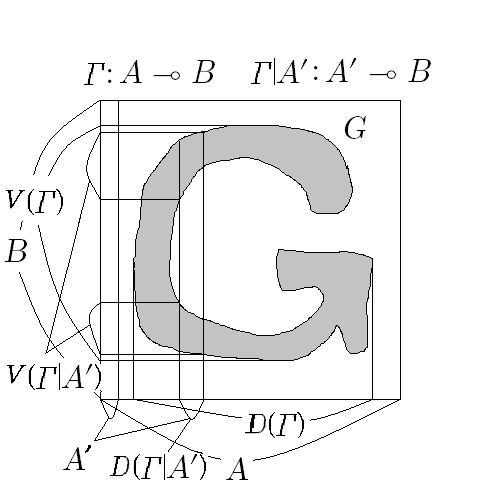
\includegraphics[width=160pt]{1.2.1.a.png}
\end{center}
\begin{thm}
\label{1.2.1.17}
2つの対応たち$\varGamma:A \multimap B$、$\varDelta:A \multimap B$について、$\forall a \in A$に対し、$\varGamma\left( \left\{ a \right\} \right) = \varDelta\left( \left\{ a \right\} \right)$が成り立つならそのときに限り、$\varGamma:A \multimap B = \varDelta:A \multimap B$が成り立つ。
\end{thm}
\begin{proof}
2つの対応たち$\varGamma:A \multimap B$、$\varDelta:A \multimap B$について、$\forall a \in A$に対し、$V\left( \varGamma|\left\{ a \right\} \right) = V\left( \varDelta|\left\{ a \right\} \right)$が成り立つならそのときに限り、2つの対応たち$\varGamma:A \multimap B$、$\varDelta:A \multimap B$をそれぞれ$(A \times B,G)$、$(A \times B,H)$とおけば、次のようになる。
\begin{align*}
&\quad \forall a \in A\left[ V\left( \varGamma|\left\{ a \right\} \right) = V\left( \varDelta|\left\{ a \right\} \right) \right]\\
&\Leftrightarrow \forall a \in A\left[ \left\{ b \in B \middle| \exists a \in \left\{ a \right\}\left[ (a,b) \in G \right] \right\} = \left\{ b \in B \middle| \exists a \in \left\{ a \right\}\left[ (a,b) \in H \right] \right\} \right]\\
&\Leftrightarrow \forall a \in A\left[ \left\{ b \in B \middle| (a,b) \in G \right\} = \left\{ b \in B \middle| (a,b) \in H \right\} \right]
\end{align*}
ここで、外延性の公理より$\forall b \in \left\{ b \in B \middle| (a,b) \in G \right\}$に対し、次式が成り立つ。
\begin{align*}
b \in \left\{ b \in B \middle| (a,b) \in G \right\} \Leftrightarrow b \in \left\{ b \in B \middle| (a,b) \in H \right\}
\end{align*}
分出の公理より次のようになる。
\begin{align*}
&\quad \left( b \in \left\{ b \in B \middle| (a,b) \in G \right\} \Leftrightarrow b \in \left\{ b \in B \middle| (a,b) \in H \right\} \right)\\
&\Leftrightarrow \left( b \in B \land (a,b) \in G \Leftrightarrow b \in B \land (a,b) \in H \right)\\
&\Leftrightarrow \neg\left( \left( b \in B \land (a,b) \in G \right) \vee \left( b \in B \land (a,b) \in H \right) \right) \\ 
&\quad \vee \left( b \in B \land (a,b) \in G \land b \in B \land (a,b) \in H \right)\\
&\Leftrightarrow \neg\left( b \in B \land \left( (a,b) \in G \vee (a,b) \in H \right) \right) \vee \left( b \in B \land (a,b) \in G \land (a,b) \in H \right)\\
&\Leftrightarrow b \notin B \vee \left( (a,b) \notin G \land (a,b) \notin H \right) \vee \left( b \in B \land (a,b) \in G \land (a,b) \in H \right)\\
&\Leftrightarrow \left( b \in B \vee b \notin B \vee \left( (a,b) \notin G \land (a,b) \notin H \right) \right) \\ 
&\quad \land \left( b \notin B \vee \left( (a,b) \in G \land (a,b) \in H \right) \vee \left( (a,b) \notin G \land (a,b) \notin H \right) \right)\\
&\Leftrightarrow \left( \top \vee \left( (a,b) \notin G \land (a,b) \notin H \right) \right) \\
&\quad \land \left( b \notin B \vee \neg\top \vee \left( (a,b) \in G \land (a,b) \in H \right) \vee \left( (a,b) \notin G \land (a,b) \notin H \right) \right)\\
&\Leftrightarrow b \notin B \vee \neg\left( b \in B \land (a,b) \in G \right) \vee \left( (a,b) \in G \land (a,b) \in H \right) \vee \left( (a,b) \notin G \land (a,b) \notin H \right)\\
&\Leftrightarrow \neg\left( b \in B \land (a,b) \in G \right) \vee \neg\left( (a,b) \in G \vee (a,b) \in H \right) \vee \left( (a,b) \in G \land (a,b) \in H \right)\\
&\Leftrightarrow \neg\top \vee \neg\left( (a,b) \in G \vee (a,b) \in H \right) \vee \left( (a,b) \in G \land (a,b) \in H \right)\\
&\Leftrightarrow \neg\left( (a,b) \in G \vee (a,b) \in H \right) \vee \left( (a,b) \in G \land (a,b) \in H \right)\\
&\Leftrightarrow \left( (a,b) \in G \Leftrightarrow (a,b) \in H \right)
\end{align*}
以上より、2つの集合たち$A$、$B$が与えられれば、直積$A \times B$も一意的に存在するので、次のようになる。
\begin{align*}
&\quad \forall a \in A\left[ V\left( \varGamma|\left\{ a \right\} \right) = V\left( \Delta|\left\{ a \right\} \right) \right]\\
&\Leftrightarrow \forall a \in A\forall b \in \left\{ b \in B \middle| (a,b) \in G \right\}\left[ (a,b) \in G \Leftrightarrow (a,b) \in H \right]\\
&\Leftrightarrow \forall a \in A\forall b \in B\left[ (a,b) \in G \Leftrightarrow (a,b) \in H \right]\\
&\Leftrightarrow \forall(a,b) \in A \times B\left[ (a,b) \in G \Leftrightarrow (a,b) \in H \right]
\end{align*}
外延性の公理より次のようになる。
\begin{align*}
\forall a \in A\left[ V\left( \varGamma|\left\{ a \right\} \right) = V\left( \varDelta|\left\{ a \right\} \right) \right] \Leftrightarrow G = H
\end{align*}
その直積$A \times B$が一意的に存在するので、したがって、$A \times B = A \times B$かつ$G = H$が成り立ち、これが成り立つならそのときに限り、$(A \times B,G) = (A \times B,H)$が成り立つ。対応の定義より、よって、2つの対応たち$\varGamma:A \multimap B$、$\varDelta:A \multimap B$について、$\forall a \in A$に対し、$\varGamma\left( \left\{ a \right\} \right) = \varDelta\left( \left\{ a \right\} \right)$が成り立つならそのときに限り、$\varGamma:A \multimap B = \varDelta:A \multimap B$が成り立つ。
\end{proof}
\begin{dfn}
対応$\varGamma:A \multimap B = (A \times B,G)$において、$\forall(a,b) \in A \times B$に対し、$(a,b) \in G \Leftrightarrow (b,a) \in H$となるような対応$(B \times A,H)$も考えられることができ、これをその対応$\varGamma:A \multimap B$の逆対応といい$\varGamma^{- 1}:B \multimap A$と書く。ここで、その対応$\varGamma^{- 1}$によるその集合$B$の部分集合$B'$の像$V\left( \varGamma^{- 1}|B' \right)$をその対応$\varGamma$によるその集合$B'$の原像、逆像などという。
\end{dfn}
\begin{thm}
\label{1.2.1.18}
対応$\varGamma:A \multimap B = (A \times B,G)$において、これの逆対応$\varGamma^{- 1}$が$\varGamma^{- 1}:B \multimap A = (B \times A,H)$と与えられたとき、$H = \left\{ (b,a) \in B \times A \middle| (a,b) \in G \right\}$が成り立つ。
\end{thm}
\begin{proof}
対応$\varGamma:A \multimap B = (A \times B,G)$において、これの逆対応$\varGamma^{- 1}$が$\varGamma^{- 1}:B \multimap A = (B \times A,H)$と与えられたとき、定義より明らかに$H \subseteq B \times A$が成り立つので、$(b,a) \in B \times A$も成り立つ。したがって、$\forall(b,a) \in H$に対し、$(a,b) \in G \Leftrightarrow (b,a) \in H$が成り立つことに注意すれば、
\begin{align*}
(b,a) \in H &\Leftrightarrow (b,a) \in B \times A \land (b,a) \in H\\
&\Leftrightarrow (b,a) \in \left\{ (b,a) \in B \times A \middle| (b,a) \in H \right\}\\
&\Leftrightarrow (b,a) \in \left\{ (b,a) \in B \times A \middle| (a,b) \in G \right\}
\end{align*}
外延性の公理より、よって、次式が成り立つ。
\begin{align*}
H = \left\{ (b,a) \in B \times A \middle| (a,b) \in G \right\}
\end{align*}
\end{proof}
%\hypertarget{ux5199ux50cf}{%
\subsubsection{写像}%\label{ux5199ux50cf}}
\begin{dfn}
対応$f:A \multimap B$について、$\forall a \in A\exists b \in B$に対し、$V\left( f|\left\{ a \right\} \right) = \left\{ b \right\}$が成り立つとき、その対応$f$は写像といい$f:A \rightarrow B$、$A\overset{f}{\rightarrow}B$などと書く。この写像$f:A \rightarrow B$全体の集合を$\mathfrak{F}(A,B)$、$B^{A}$などと書く。このとき、$V\left( f|\left\{ a \right\} \right) = \left\{ b \right\}$のことを、単に、$f(a) = b$と書き、これを明示するとき、その写像$f$を$f:A \rightarrow B;a \mapsto f(a) = b$などと書くときがありその元$b$をその元$a$のその写像$f$による像、その元$a$におけるその写像$f$の値などといいこのことをその写像$f$はその元$a$をその元$b$に写す、その元$a$にその元$b$を対応させるなどという。
\end{dfn}
これらの用語たちは次の図のように該当される。
\begin{center}
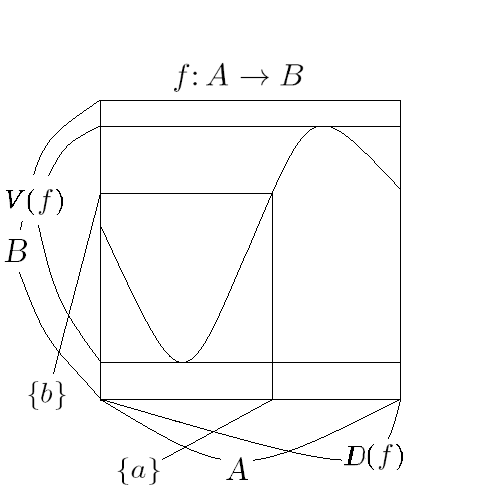
\includegraphics[width=160pt]{1.2.1.b.png}
\end{center}
%\hypertarget{ux4e00ux822cux5316ux3055ux308cux305fux76f4ux7a4d}{%
\subsubsection{一般化された直積}%\label{ux4e00ux822cux5316ux3055ux308cux305fux76f4ux7a4d}}
\begin{dfn}
空でない集合$\varLambda$と集合$A$を用いて、写像$a:\varLambda \rightarrow A$を考えるとき、順序対$\left( a,V(a) \right)$をその集合$\varLambda$によって添数づけられた集合といい、その集合$\varLambda$をその集合$\left( a,V(a) \right)$の添数集合、これの元$\lambda$を添数という。ここで、$a(\lambda)$を$a_{\lambda}$とも書き、その値域$V(a)$は$\left\{ a_{\lambda} \in A \middle| \lambda \in \varLambda \right\}$とも書かれることができる。これをその集合$A$の集合族などといい単に$\left\{ a_{\lambda} \middle| \lambda \in \varLambda \right\}$、$\left\{ a_{\lambda} \right\}_{\lambda \in \varLambda}$などとも書く。
\end{dfn}
\begin{dfn}
次式で定義される集合$\prod_{\lambda \in \varLambda} A_{\lambda}$を空でない集合$\varLambda$によって添数づけられた族$\left\{ A_{\lambda} \right\}_{\lambda \in \varLambda}$の一般化された直積という。なお、集合$\mathfrak{F}\left( \varLambda,\bigcup_{\lambda \in \varLambda} A_{\lambda} \right)$に属する写像$f$を用いた集合$f(\lambda)$が$a_{\lambda}$にあたる。
\begin{align*}
\prod_{\lambda \in \varLambda} A_{\lambda} = \left\{ f \in \mathfrak{F}\left( \varLambda,\bigcup_{\lambda \in \varLambda} A_{\lambda} \right) \middle| \forall\lambda \in \varLambda\left[ f(\lambda) \in A_{\lambda} \right] \right\}
\end{align*}
\end{dfn}
これにより、その写像$f$を$\left( a_{\lambda} \right)_{\lambda \in \varLambda}$と書くことがある。\par
特に、のちに述べるように、$\varLambda = \left\{ \mu,\nu \right\}$、$A_{\mu} = A$、$A_{\nu} = B$、$f(\mu) = a$、$f(\nu) = b$とすれば、その直積$\prod_{\lambda \in \varLambda} A_{\lambda}$、その写像$f$をそれぞれ$A \times B$、$(a,b)$と書くこともある。
\begin{thm}
\label{1.2.1.19}
$f \in \prod_{\lambda \in \varLambda} A_{\lambda}$が成り立つならそのときに限り、写像$f:\varLambda \rightarrow \bigcup_{\lambda \in \varLambda} A_{\lambda}$が与えられ、$\forall\lambda \in \varLambda$に対し、$f(\lambda) \in A_{\lambda}$が成り立つ。
\end{thm}
\begin{proof}
空でない集合$\varLambda$によって添数づけられた族$\left\{ A_{\lambda} \right\}_{\lambda \in \varLambda}$の一般化された直積$\prod_{\lambda \in \varLambda} A_{\lambda}$が与えられたとする。定義より次式が成り立つので、
\begin{align*}
\prod_{\lambda \in \varLambda} A_{\lambda} = \left\{ f \in \mathfrak{F}\left( \varLambda,\bigcup_{\lambda \in \varLambda} A_{\lambda} \right) \middle| \forall\lambda \in \varLambda\left[ f(\lambda) \in A_{\lambda} \right] \right\}
\end{align*}
$f \in \prod_{\lambda \in \varLambda} A_{\lambda}$が成り立つなら、次式が成り立ち、
\begin{align*}
f \in \left\{ f \in \mathfrak{F}\left( \varLambda,\bigcup_{\lambda \in \varLambda} A_{\lambda} \right) \middle| \forall\lambda \in \varLambda\left[ f(\lambda) \in A_{\lambda} \right] \right\}
\end{align*}
分出の公理より写像$f:\varLambda \rightarrow \bigcup_{\lambda \in \varLambda} A_{\lambda}$が与えられ、$\forall\lambda \in \varLambda$に対し、$f(\lambda) \in A_{\lambda}$が成り立つ。\par
逆に、これが成り立つなら、$f \in \mathfrak{F}\left( \varLambda,\bigcup_{\lambda \in \varLambda} A_{\lambda} \right)$かつ、$\forall\lambda \in \varLambda$に対し、$f(\lambda) \in A_{\lambda}$が成り立つので、分出の公理より次式が成り立ち、
\begin{align*}
f \in \left\{ f \in \mathfrak{F}\left( \varLambda,\bigcup_{\lambda \in \varLambda} A_{\lambda} \right) \middle| \forall\lambda \in \varLambda\left[ f(\lambda) \in A_{\lambda} \right] \right\}
\end{align*}
したがって、$f \in \prod_{\lambda \in \varLambda} A_{\lambda}$が成り立つ。
\end{proof}
\begin{thm}
\label{1.2.1.20}
このように定義してもなお、$\varLambda = \left\{ \mu,\nu \right\}$、$A_{\mu} = A$、$A_{\nu} = B$とすれば、$\forall f,g \in A \times B$に対し、$f = g$が成り立つならそのときに限り、$\left( f(\mu),f(\nu) \right) = \left( g(\mu),g(\nu) \right)$が成り立つ。
\end{thm}
\begin{proof}
$\varLambda = \left\{ \mu,\nu \right\}$、$A_{\mu} = A$、$A_{\nu} = B$とすれば、$\forall f,g \in A \times B$に対し、次のようになる。
\begin{align*}
f = g &\Leftrightarrow \forall\lambda \in \varLambda\left[ f(\lambda) = g(\lambda) \right]\\
&\Leftrightarrow f(\mu) = g(\mu) \land f(\nu) = g(\nu)\\
&\Leftrightarrow \left( f(1),f(2) \right) = \left( g(1),g(2) \right)
\end{align*}
\end{proof}
\begin{thm}
\label{1.2.1.21}
空でない集合$\varLambda$によって添数づけられた族$\left\{ A_{\lambda} \right\}_{\lambda \in \varLambda}$の直積$\prod_{\lambda \in \varLambda} A_{\lambda}$において、$\prod_{\lambda \in \varLambda} A_{\lambda} \neq \emptyset$が成り立つなら、$\forall\lambda \in \varLambda$に対し、$A_{\lambda} \neq \emptyset$が成り立つ。
\end{thm}
\begin{proof}
空でない集合$\varLambda$によって添数づけられた族$\left\{ A_{\lambda} \right\}_{\lambda \in \varLambda}$の直積$\prod_{\lambda \in \varLambda} A_{\lambda}$において、$A_{\lambda'} = \emptyset$が成り立つような$\lambda'$が存在するかつ、その直積$\prod_{\lambda \in \varLambda} A_{\lambda}$が空集合でないとすると、直積の定義より$f\left( \lambda' \right) \in A_{\lambda'}$となるような元$f$が存在することになるが、これは$A_{\lambda'} = \emptyset$に矛盾する。したがって、$A_{\lambda'} = \emptyset$が成り立つような$\lambda'$が存在する、即ち、$\exists\lambda' \in \varLambda$に対し、$A_{\lambda'} = \emptyset$が成り立つなら、その直積$\prod_{\lambda \in \varLambda} A_{\lambda}$が空集合である、即ち、$\prod_{\lambda \in \varLambda} A_{\lambda} = \emptyset$が成り立つ。あとは対偶律による。
\end{proof}
%\hypertarget{ux9078ux629eux306eux516cux7406}{%
\subsubsection{選択の公理}%\label{ux9078ux629eux306eux516cux7406}}
\begin{axs}
次式で表される公理を選択の公理、選択公理、選出公理などという。
\begin{align*}
\forall\mathcal{A}\in \mathcal{F\exists}f \in \mathfrak{F}\left( \mathcal{A},\bigcup_{} \mathcal{A} \right)\forall A \in \mathcal{A}\left[ A \neq \emptyset \Rightarrow f(A) \in A \right]
\end{align*}
\end{axs}
これはどの集合$\mathcal{A}$でも、その集合$\mathcal{A}$に属する空でない任意の元$A$に対し、$f(A) \in A$となるような写像$f:\mathcal{A} \rightarrow \bigcup_{} \mathcal{A}$が存在するという意味である。この写像$f$をその集合$\mathcal{A}$の選択写像などという。\footnote{この公理はその写像の具体的な構成が言及されておらず、しばしば直感に反するような命題を導くことがあり、この公理が取り除かれたり、含められたりしたとしても矛盾は生じないと知られているが、この公理が取り除かれると、さまざまな定理たちが証明されることができなくなってしまうため、この公理も含めることが多い…とはいったものの、選択の公理なんか認めん! とかいっていたら数学者の中では異端児扱いされるらしい(?)。}
\begin{thm}
\label{1.2.1.22}
空でない集合$\varLambda$によって添数づけられた族$\left\{ A_{\lambda} \right\}_{\lambda \in \varLambda}$の直積$\prod_{\lambda \in \varLambda} A_{\lambda}$において、$\forall\lambda \in \varLambda$に対し、$A_{\lambda} \neq \emptyset$が成り立つならそのときに限り、$\prod_{\lambda \in \varLambda} A_{\lambda} \neq \emptyset$が成り立つ。
\end{thm}
\begin{proof}
空でない集合$\varLambda$によって添数づけられた族$\left\{ A_{\lambda} \right\}_{\lambda \in \varLambda}$の直積$\prod_{\lambda \in \varLambda} A_{\lambda}$において、$\prod_{\lambda \in \varLambda} A_{\lambda} \neq \emptyset$が成り立つなら、$\forall\lambda \in \varLambda$に対し、$A_{\lambda} \neq \emptyset$が成り立つのであった。逆に、$\forall\lambda \in \varLambda$に対し、$A_{\lambda} \neq \emptyset$が成り立つなら、一般化された直積の定義より、写像$f:\varLambda \rightarrow \left\{ A_{\lambda} \right\}_{\lambda \in \varLambda};f(\lambda) = A_{\lambda}$が存在するのであった。選択の公理よりその集合$\left\{ A_{\lambda} \right\}_{\lambda \in \varLambda}$の選択写像を$g$とすれば、$g\left( A_{\lambda} \right) \in A_{\lambda}$が成り立つ。ここで、写像$h:\varLambda \rightarrow \bigcup_{} \left\{ A_{\lambda} \right\}_{\lambda \in \varLambda} = \bigcup_{\lambda \in \varLambda} A_{\lambda};\lambda \mapsto g\left( A_{\lambda} \right) = g\left( f(\lambda) \right)$を考えると、$h(\lambda) \in A_{\lambda}$が成り立つので、$h \in \prod_{\lambda \in \varLambda} A_{\lambda}$が成り立つ。
\end{proof}
\begin{thebibliography}{50}
    \bibitem{1}
      Rei Frontier Tech Blog. "ZFC公理系について:その1". Hatena Blog. \url{https://tech-blog.rei-frontier.jp/entry/2017/11/02/102042}, (2021-04-01 20:30 閲覧)
    \bibitem{2}
      Rei Frontier Tech Blog. "ZFC公理系について:その2". Hatena Blog. \url{https://tech-blog.rei-frontier.jp/entry/2017/11/09/100000}, (2021-04-01 20:30 閲覧)
    \bibitem{3}
      Rei Frontier Tech Blog. "ZFC公理系について:その3". Hatena Blog. \url{https://tech-blog.rei-frontier.jp/entry/2017/11/16/100000} (2021-04-01 20:30 閲覧)
\end{thebibliography}
\end{document}
    
